\chapter{System Architecture} \label{ch:SysArchitecture}

A proposal for a system architecture for an impedance analyzer had been made based on the system requirements listed in section \refq{ch:SystemRequirements}. The architecture can be seen on the block diagram on figure \refq{fig_6_SysArchitecture}.  

\begin{figure}[H]
    \centering
    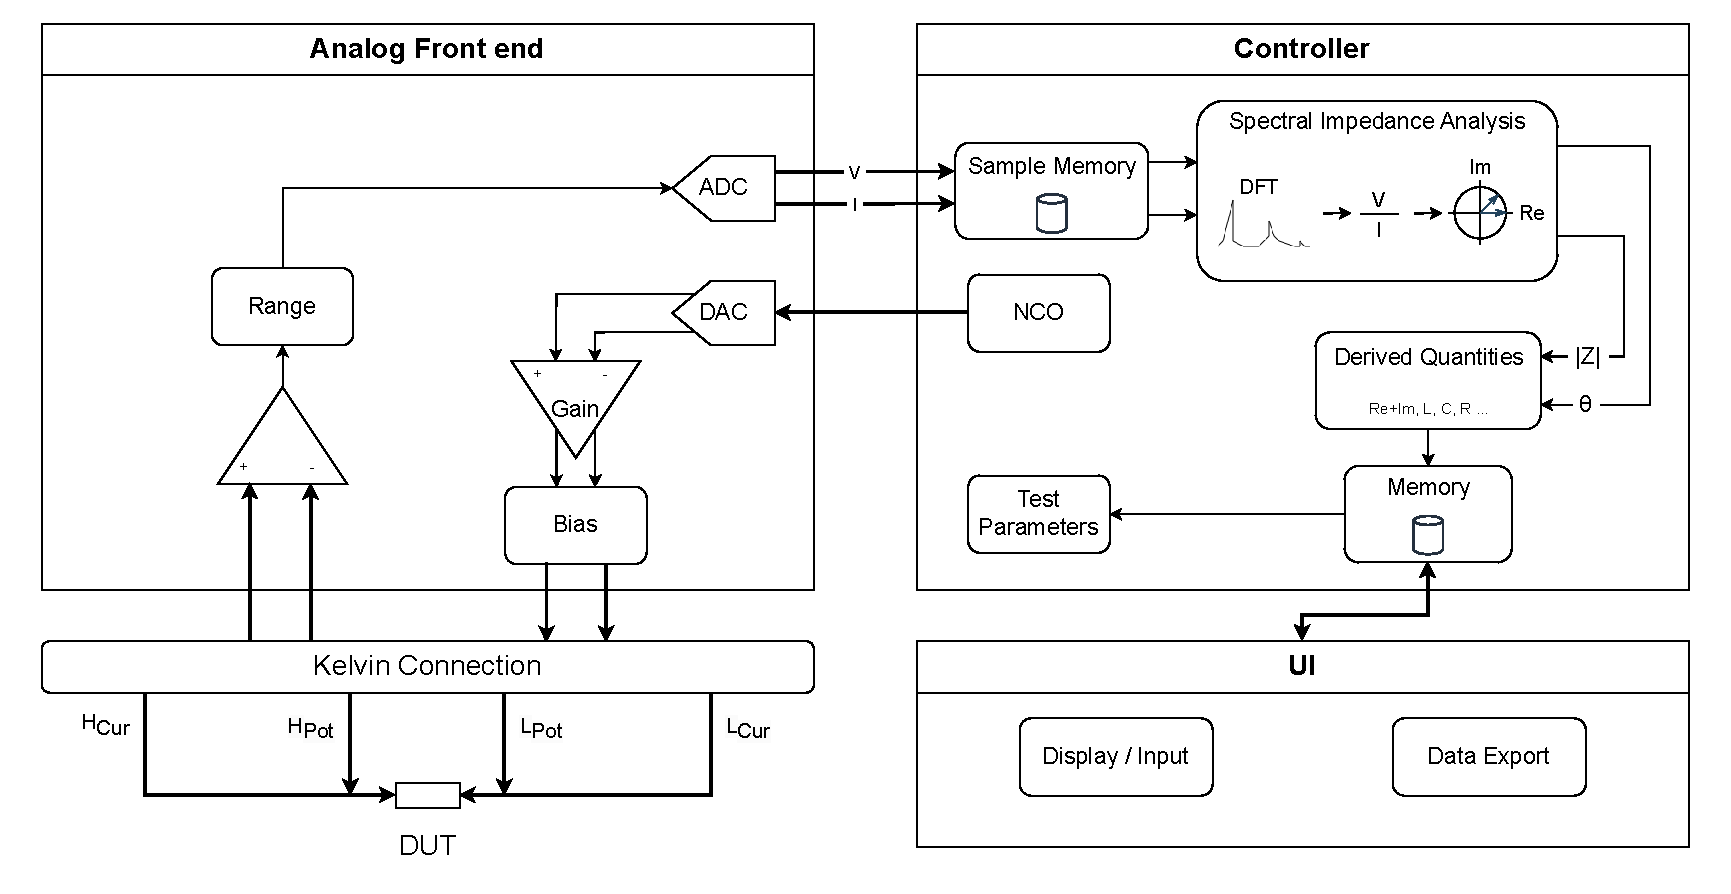
\includegraphics[clip, trim=18 0 18 0,width=1.0\textwidth]{Sections/6_SystemArchitecture/Figures/SystemArchitecture.pdf}
    \caption{The proposed system architecture for the impedance analyzer designed in this document. An analog front end will measure DUT voltage and current, 
    this will then undergo spectral analysis, such that phase and magnitude information can be obtained and used to calculate all derived quantities. A user can set the test parameters using a UI, these parameters in turn will determine DAC settings, range and sample rate.}
    \label{fig_6_SysArchitecture}
\end{figure}

The impedance analyzer will be designed around the two major blocks on figure \refq{fig_6_SysArchitecture}, namely an analog front end and a control system. The analog front end is a major part of the impedance analyzer, it is responsible for generating the test signals for the DUT with DA-conversion and sampling the resulting DUT current and voltage waveforms with AD-conversion. The reconstruction and anti-aliasing filters are not shown on the figure but is assumed to be there.

A kelvin connection (4-wire) will be used to connect the DUT to an analog front end. This connection uses two pairs of connections, one pair carries a high current and the other measures the voltage at the DUT. This connection allows the system to compensate for impedance in the high current leads and resistance in the DUT contacts.

A DAC will generate the test signals for the DUT through a programmable gain amplifier to ensure that the ADC always samples as large current and voltage signals as possible. This will allow the system to make use the ADC's full dynamic range and increase the signal-to-noise ratio. The DAC \textit{side} of the analog front end will have a system to DC bias the DUT as well, this means the DUT will see a sum of the test signal and DC bias voltage. The DC bias function will be described later in this report.

The ADC will sample the DUT current waveform through a MUX'ed set of range resistors. These resistors can be selected by the control system to, also, ensure that the ADC uses it's full dynamic range. A \textit{low} value range resistor may be used if the DUT impedance is low and vice versa.

The control system may be a microcontroller or FPGA, or a combination of both as will be described later. The control system will take the readings from the ADC in the analog front end and generate the clock signals for the DAC. The clock signals for the DAC must be adjustable to give the desired resolution that was described in section \refq{ch:SystemRequirements}, so the control system must have a controlled oscillator. A numerically controlled oscillator will be used for this purpose, which is either implemented on an FPGA, or a microcontroller hardware module. 

The sampled current and voltage waveforms from the analog front end will undergo spectral analysis in order to retrieve the magnitude and phase information for the DUT's impedance. This impedance will then be converted into the derived quantities described in section \refq{subsec:DerivedQuantities}. The derived quantities will be stored in memory and the \textit{UI} block is responsible to displaying this data to the user. The UI block is a display, possibly touchscreen, that will allow the user to set all the required test parameters and sweep settings. The UI will also have a way to export data to the user, either over UART, USB or similar. 
